\documentclass[10pt,aspectratio=169]{beamer}
%\setbeameroption{show notes on second screen=right}

%\usetheme{Madrid}


\usetheme[progressbar=frametitle]{metropolis}
\usecolortheme{rose} %beaver, dolphin, crane, 


\setbeamersize{text margin left=4mm, text margin right=4mm}


\usecolortheme{default}
\setbeamertemplate{navigation symbols}{}
\setbeamertemplate{footline}[frame number]
\usepackage[utf8]{inputenc}
\usepackage[T1]{fontenc}

\usepackage{amsmath, amssymb, bm}
\usepackage{booktabs}
\usepackage{graphicx}
\usepackage{ragged2e}
\usepackage{hyperref}
%\hypersetup{colorlinks=true, urlcolor=blue}


\AtBeginSection[]
{
  \begin{frame}{Outline}
    \tableofcontents[currentsection]%,hideothersubsections]
  \end{frame}
}

\setbeamercolor{item}{fg= orange!80} % Change bullet color
\setbeamercolor{button}{bg=orange, fg=white}

\title[Competing under Information Heterogeneity]{Competing under Information Heterogeneity:\\ Evidence from Auto Insurance}
\author[Cosconati, Fan, Jin, Wu]{Marco Cosconati \and Yi Xin  \and Yizhou Jin \and Fan Wu}
\institute{IVASS, Bank of Italy \and Caltech \and Caltech \and University of Toronto}
\date{July 8, 2025}

\begin{document}

% 1
\begin{frame}
  \titlepage
\end{frame}

% 2
\begin{frame}{Motivation}
\justifying
\begin{itemize}
  \item Firms increasingly differ in \emph{information precision} (data access/analytics) and in \emph{cost structures}.
  \item This creates information asymmetries \emph{between} firms (beyond classic buyer--seller asymmetry).
  \item Policy interest: regulations that equalize or share consumer risk information (e.g., centralized ``risk bureau'', Open Banking policies).
\end{itemize}
\end{frame}

% 3 - This paper
\begin{frame}{This paper}
\begin{itemize}
  \item Research Questions
  
  \begin{itemize}
  \item How does heterogeneous information across insurers shape market equilibrium? %pricing, sorting, and market power?
  \item What are the equilibrium impacts of establishing a centralized bureau to equalize information access?
  \end{itemize} 
  \item Contributions
  \begin{itemize}
  \item A tractable model of imperfect competition with firm-specific information precision and costs.
  \item New identification/estimation strategy using offered-price distributions and demand to recover signals.
  \item Evidence from Italian auto liability insurance with rich panel linking consumers across insurers.
  \item Counterfactuals: centralized risk bureau, full information, and privacy/high-variance restrictions.
\end{itemize}
\end{itemize}
\end{frame}

% 4 - Literature
\begin{frame}{Literature}
\begin{enumerate}
  \item Selection markets 
  \begin{itemize}
    \item Competitive models: Einav et al. (2010, 2011), Azevedo \& Gottlieb (2017); Assymmetric information: Cabral et al. (2018), Crawford et al. (2018), Cuesta et al. (2021) and Tebaldi (2024)
    
    $\rightarrow$ Incorporates multidimensional cost heterogeneity
  \end{itemize}
  \item Demand estimation 
  \begin{itemize}
    \item Berry (1994),  BLP(1995) and  D'Haultfœuille et al. (2019) 
    
    $\rightarrow$ Extends demand estimation when prices are not observed. 
  \end{itemize}
  
  \item Antitrus/Consumer protection and Big Data  
  \begin{itemize}
    \item Einav et al. (2013), Chatterjee et al. (2023), Blattner \& Nelson (2021), Lam \& Liu (2020), Jin \& Wagman (2021)
    
    $\rightarrow$ Policies that equalize information access can improve competition
  \end{itemize}
\end{enumerate}
\end{frame}


 
%%%%%%%%%%%%%%%%%%%%%%%%%%%%%%%%%%%%%%%%%%%%%%%%%%%%
\section{Setting and Data}

% 5 - Institutional Background
\begin{frame}{Institutional Background: Italian Auto Liability (RCA)}
\justifying
\begin{itemize}
  \item Mandatory, annual, exclusive contracts; insurers cannot reject consumers.
  \item Large market: $\approx$31M contracts in 2018; $\approx$50 national competitors.
  \item Key contract features widely standardized; little use of deductibles.
\end{itemize}
\end{frame}

% 6 - Data
\begin{frame}{Data: IVASS IPER Microdata}
\justifying
\begin{itemize}
  \item Nationally representative matched insurer--insuree panel with claims frequency/severity, premiums, coverage.
  \item Tracks policyholders across insurers and time $\Rightarrow$ measure risk using ex-post claims panel.
  \item Focus sample: new customers in Rome (2013--2021); top 10 firms + fringe group.
\end{itemize}
\end{frame}

%%%%%%%%%%%%%%%%%%%%%%%%%%%%%%%%%%%%%%%%%%%%%%%%%%%
\section{Descriptive evidence}

% 9 - Sample and Summary Statistics
\begin{frame}{Sample \& Summary Statistics}
\justifying
\begin{itemize}
  \item $N \approx 124{,}428$ contracts; avg premium $\approx \,€478$; within-year claim rate $\approx 0.08$.
  \item Demographics/vehicle: 56\% male; avg age 48; BM class $\approx 2$; car age $\approx 8.3$ years.
\end{itemize}
\begin{figure}[H]
\centering{}%
\begin{tabular}{cc}
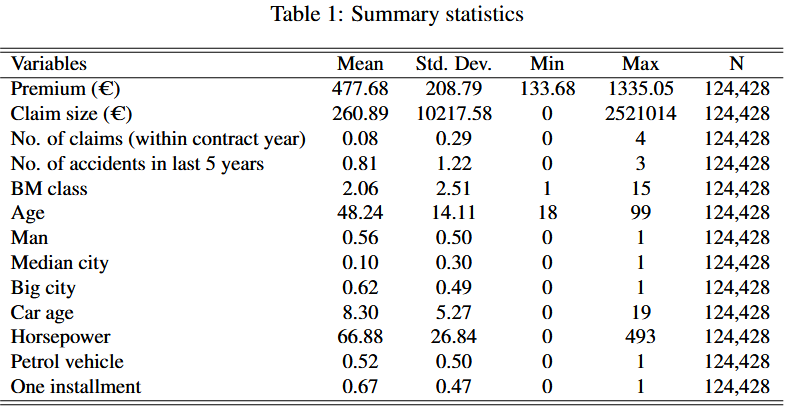
\includegraphics[scale=0.45]{Figures/Tab1.png}
\end{tabular}
\end{figure}
\end{frame}

% 10 - Stylized Facts
\begin{frame}{Stylized Facts: Price Variation \& Sorting}
\begin{figure}[H]
\centering{}%
\begin{tabular}{cc}
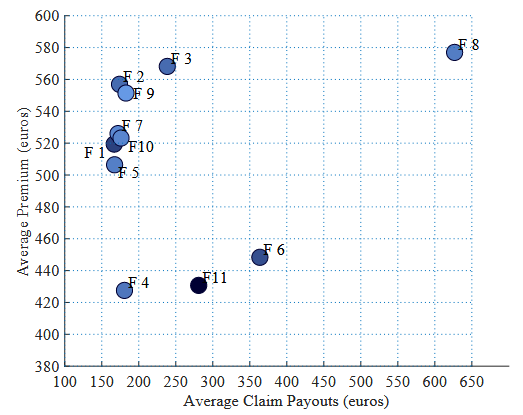
\includegraphics[scale=0.47]{Figures/Fig1.png}
\end{tabular}
\end{figure}
\vspace{0.75em}
\begin{itemize}
  \item Large cross-firm variation in average premiums even at similar average risks/market shares.
  \item Firms with higher average claim costs attract riskier consumers $\Rightarrow$ sorting across firms.
\end{itemize}
\end{frame}

% 11 - Measuring Information Precision
\begin{frame}{Measuring Information Precision}
\begin{enumerate}
\item Step 1: Construct individual risk measures
\begin{itemize}
\item Panel regression of claim counts and size  with individual fixed effects
%\item Log-normal regression of claim severity conditional on accident
\item Risk measure = $ \underbrace{\exp(X_{it}\delta_c + \zeta_i)}_{\text{Claim Count}} \cdot  \underbrace{\exp(\delta_0 + X_{it}+ \eta_{it})}_{\text{Claim Size}}$
\end{itemize}
\item Step 2: Firm-specific premium-risk regressions
\begin{itemize}
\item For each firm $j$: $\text{Premium}_{ij} = \alpha_j + \beta_j \cdot \text{Risk}_i + \varepsilon_{ij}$
\item Higher $\beta_j$ suggests firm's prices are more responsive to actual risk
\end{itemize}
\end{enumerate}
\end{frame}

% 12 - Heterogeneity in Risk Sensitivity
\begin{frame}{Heterogeneity in Risk Sensitivity}
\justifying
\begin{itemize}
  %\item Measure how strongly each firm’s premium responds to realized consumer risk (ex-post panel-based risk).
  \item Strong cross-firm differences in premium–risk slopes $\Rightarrow$ heterogeneous precision? 
  \item Prices are equilibrium outcomes $\Rightarrow$ need structural model to recover information precision.
\end{itemize}
\vspace{0.75em}
\begin{figure}[H]
\centering{}%
\begin{tabular}{cc}
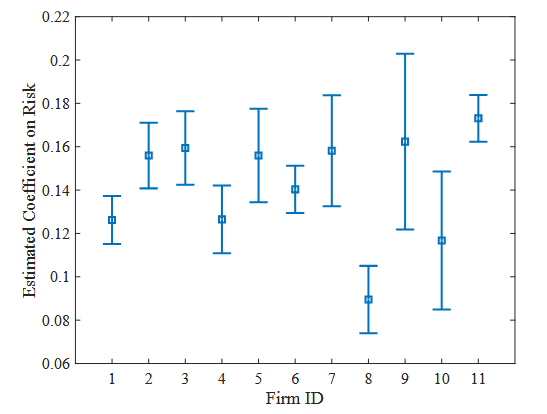
\includegraphics[scale=0.45]{Figures/Fig2.png}
\end{tabular}
\end{figure}
\note{Given that prices are equilibrium outcomes for example we could have that the patterns observed in the data are demand driven}
\end{frame}

%%%%%%%%%%%%%%%%%%%%%%%%%%%%%%%%%%%%%%%%%%%%%%%%%%%
\section{Model}

% 14
\begin{frame}{Model overview}
\justifying
\begin{itemize}
  \item $J$ insurers; standardized product; no outside option.
  \item Consumer true risk $\theta$ (expected cost/year) unobserved ex ante.
  \item Firm $j$ observes a private signal $\hat{\theta}_j$ with precision that differs across firms.
  \item $D$ denotes the contract chosen by the consumer.
\end{itemize}
\end{frame}

% 15 - Signal Structure
\begin{frame}{Signal Structure}
\justifying
\begin{equation}
\hat{\theta}_j \sim \mathcal{N}(\theta,\ \sigma_j^2), \quad \text{iid}  
\label{eq:signal}
\end{equation}
\begin{itemize}
  \item Denote by $\phi(\hat{\theta}_j \mid \theta, \sigma_j)$ the density
  \item Lower $\sigma_j^2$ $\Rightarrow$ higher information precision for firm $j$.
  \item Signals are used to form posterior beliefs about $\theta$ \emph{conditional on selection}.

\begin{align}
  E(\theta | \hat{\theta}_j, D=j) = \int_{\theta} \theta f(\theta | \hat{\theta}_j, D=j) d\theta = \frac{\int_{\theta} \theta \overbrace{\Pr(D=j | \hat{\theta}_j, \theta)}^{\text{Selection Prob.}} \phi(\hat{\theta}_j; \theta, \sigma_j) f_0(\theta) d\theta}{\int_{\theta} \Pr(D=j | \hat{\theta}_j, \theta) \phi(\hat{\theta}_j; \theta, \sigma_j) f_0(\theta) d\theta}  
\end{align}
\end{itemize}
\note{Emphasize that the probability of choosing given type and signals is an equilibrium object. }
\end{frame}

% 16 - Pricing
\begin{frame}{Pricing}
\begin{itemize}
\item Assumes: 
  \begin{equation}
p_j(\hat{\theta}_j) \;=\; \alpha_j \;+\; \beta_j \, \mathbb{E}[\theta \mid \hat{\theta}_j,\, D=j],
\end{equation}
  \item $\alpha_j$: baseline markup; $\beta_j$: sensitivity to risk rating.
  \item $\mathbb{E}[\theta \mid \hat{\theta}_j, D=j]$ embeds selection $\Rightarrow$ nonlinearity in $\hat{\theta}_j$.
\end{itemize}
\end{frame}

% 17 - Demand
\begin{frame}{Demand}
\justifying
\begin{itemize}
  \item Consumers choose one insurer (no outside option); utility depends on price and observable characteristics.
  \item Preference parameters allowed to vary with observables and risk type. Consumer $i$'s utility from firm $j$:
\end{itemize}
\begin{align}
  U_{ij} = -\gamma(\theta)p_j(\tilde{\theta}_j) + \xi_j(\theta) + \varepsilon_{ij} 
\end{align}
\begin{align}
  \Pr(D=j|\hat{\theta}, \theta) = \frac{\exp(-\gamma(\theta)p_j(\hat{\theta}_j) + \xi_j(\theta))}{\sum_{j'=1}^{J}\exp(-\gamma(\theta)p_{j'}(\hat{\theta}_{j'}) + \xi_{j'}(\theta))} 
\end{align}
\end{frame}

% 18 - Firm profits
\begin{frame}{Firm profits}
    \begin{itemize}
        \item Firms simultaneously choose pricing coefficients $(\alpha_j, \beta_j)$ to maximize expected profits, given common knowledge of all firms' primitives (e.g., signal distributions, costs) and $f_0(\theta)$.
        
        \medskip
        \item Firm $j$'s profit 
        
        \[\pi_j(\alpha, \beta) = 
        \int_{\hat{\theta}} \int_{\theta} \underbrace{(p_j(\hat{\theta}_j) + c_j - k_j\theta)}_{\text{net profit}} \underbrace{\Pr(D=j|\hat{\theta})}_{\text{choice prob.}} \underbrace{\left(\prod_{j'=1}^{J} \phi(\hat{\theta}_{j'}; \theta, \sigma_{j'}) \right)}_{\text{signal dist.}} \underbrace{f_0(\theta)}_{\text{type dist.}} d\theta d\hat{\theta}.
        \]
        
        \medskip
        \item $c_j$: ``net benefits'' of contracting with a customer irrespective of the risk.
        
        \item $k_j$: efficiency at processing claims.
    \end{itemize}
\end{frame}


%%%%%%%%%%%%%%%%%%%%%%%%%%%%%%%%%%%%%%%%%%%%%%%%%%%
\section{Estimation}

% 20 - Estimation Overview
\begin{frame}{Estimation Overview}\label{estimation:overview}
  \begin{itemize}
    \item Joint distribution of premium and risk types  \hyperlink{appendix:slide1}{\beamergotobutton{Details}}
    \begin{itemize}
      \item Uses panel of claim records
      \item Claim size estimated via regression
      \item Accident rate identified from panel of accident counts (repeated noisy measurements)
      \item Output   $\hat{g}(p | \theta, D=j)$
  \end{itemize}
    \item Demand ($\gamma(\theta), \xi_j(\theta)$)
    \begin{itemize}
      \item $\xi_j(\theta)$: matched to observed market shares
      \item $\gamma(\theta)$: identified from sorting patterns
    \end{itemize}
    \item Supply ($\alpha_j, \beta_j, \sigma_j^2, c_j, k_j$)
    \begin{itemize}
      \item Average price conditional on risk identifies $(\alpha_j, \beta_j)$  \hyperlink{appendix:slide3}{\beamergotobutton{Details}}
      \item $\sigma_j$ is identified from price dispersion given risk  \hyperlink{appendix:slide3.1}{\beamergotobutton{Details}}
      \item Cost parameters $(c_j, k_j)$ recovered from first-order conditions \hyperlink{appendix:slide4}{\beamergotobutton{Details}}
    \end{itemize}
  \end{itemize}
\end{frame}


% 21 - Demand estimation
 \begin{frame}{Demand Estimation}\label{estimation:demand}
\begin{columns}[t]
\begin{column}{0.51\textwidth}
\textbf{Challenge:}
\begin{itemize}
    \item Observe \textbf{accepted prices}, not offered prices
    \item Lower prices over-represented in data
\end{itemize}

\vspace{0.3cm}
\textbf{Solution:}
\begin{itemize}
    \item Use selection rule (demand model) to recover distribution of offered prices
\end{itemize}

\vspace{0.2cm}
{\small
Relationship:
$$ g(p|\theta, D=j) \propto g_j(p|\theta) \Pr(D=j|p_j=p, \theta) $$

Recover offered prices:
$$ g_j(p|\theta) = \frac{g(p|\theta, D=j) / \Pr(D=j|p_j=p, \theta)}{\int_{p'} g(p|\theta, D=j) / \Pr(D=j|p_j=p', \theta)dp'} $$
}
\hyperlink{appendix:slide2}{\beamergotobutton{Details}}
\end{column}
\begin{column}{0.45\textwidth}
\vspace{0.5cm}
\begin{center}
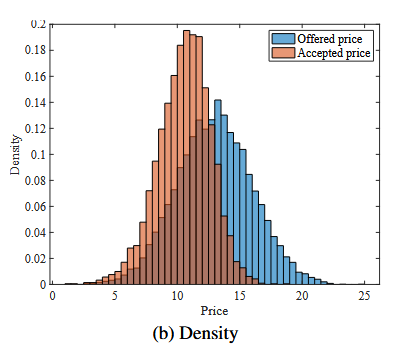
\includegraphics[width=\textwidth]{Figures/Fig3B.png}
\end{center}
\end{column}
\end{columns}
\end{frame}

% 22 - Iterative Algorithm 
\begin{frame}{Iterative Algorithm for Demand Estimation}
\small 
\textbf{Nested Fixed-Point Algorithm:} Jointly estimate sorting probabilities, price distributions, and demand parameters

\vspace{0.1cm}

\textbf{Inner Loop:} For fixed $\gamma$ (price sensitivity)

\begin{enumerate}
    \item Initialize: $\xi_j^1 = 0$ and $\Pr^1(D=j|p_j=p, \theta) = \exp(\alpha p)$ for all $j$
    
    \item Update offered-price density, using Bayes' rule: 
    {\small
    $$ g_j^r(p|\theta) = \frac{\hat{g}(p|\theta, D=j) / \Pr^r(D=j|p_j=p, \theta)}{\int_{p'} \hat{g}(p'|\theta, D=j) / \Pr^r(D=j|p_j=p', \theta)dp'} $$
    }
    
    \item Update $\xi^{r+1}$ to match observed market shares:
    {\small
    $$ \hat{s}_j = \int_\theta \int_p \frac{\exp(\alpha p_j + \xi_j^{r+1})}{\sum_{j'} \exp(\alpha p_{j'} + \xi_{j'}^{r+1})} \left(\prod_{j'} g_{j'}^r(p_{j'}|\theta)\right) f_0(\theta) dp d\theta $$
    }
    
    \item Update selection probabilities $\Pr^{r+1}(D=j|p_j=p, \theta)$ using demand model
    
    \item Iterate until $g^r$ converges. Output $\{g_j(p\mid\theta;\gamma)\}_j$, $\Pr(D=j\mid p,\theta;\gamma)$, and $\xi(\gamma)$.
\end{enumerate}

\vspace{0.2cm}

\textbf{Outer Loop:} Estimate $\alpha$ by matching risk sorting patterns via maximum likelihood

\end{frame}


\section{Results and Counterfactuals}

% 24 - Results: supply-side
\begin{frame}{Results: Supply-Side}

\begin{columns}[t]
\begin{column}{0.44\textwidth}


\begin{itemize}
  \item Large differences in information precision  ($\sigma_j^2$) and price sensitivity ($\beta_j$) across firms
    
  \item Baseline markups ($\alpha_j$) differ, consistent with market power from information advantages
  
  
  \item Large contracting net benefits (e.g., for F8 is four times average premium)
  \item Heterogeneity in claim efficiency(e.g. F8 roughly 2.5 times less efficient than F6)
\end{itemize}
\end{column}

\begin{column}{0.51\textwidth}
\vspace{-0.3cm}
\begin{figure}[H]
\centering
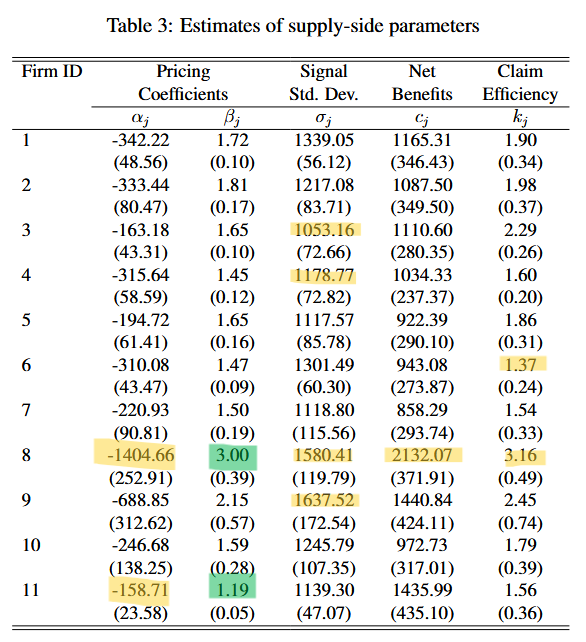
\includegraphics[width=\textwidth]{Figures/Tab3_hihglighted.png}
\end{figure}
\end{column}
\end{columns}

\end{frame}

% 25 - Results: supply-side
\begin{frame}{Results: supply-side}
\begin{itemize}
  \item More(less) precise firms, attract less(more) risky consumers
\end{itemize}
\begin{figure}[H]
\centering{}%
\begin{tabular}{cc}
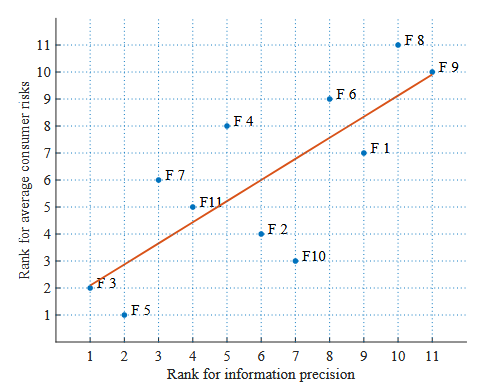
\includegraphics[scale=0.57]{Figures/Fig4.png}
\end{tabular}
\end{figure}
\end{frame}

% 26 - Counterfactuals: Information Policies
\begin{frame}{Counterfactuals: Information Policies}
\justifying
\begin{itemize}
  \item \textbf{Centralized Risk Bureau}: aggregate firms’ signals (weighted by precision), share equally with all.
  \begin{align}
  E(\theta|\hat{\theta}) = \int_{\theta} \theta f(\theta|\hat{\theta}) d\theta = \frac{\int_{\theta} \theta \left( \prod_j \phi(\hat{\theta}_j; \theta, \sigma_j) \right) f_0(\theta) d\theta}{\int_{\theta} \left( \prod_j \phi(\hat{\theta}_j; \theta, \sigma_j) \right) f_0(\theta) d\theta}
\end{align}
  \item \textbf{Full Information Benchmark}: firms observe true $\theta$ (eliminate information asymmetry).
  \item \textbf{Privacy/Restriction}: firms can only use basic information; set $\sigma_j^2$ to the worst observed.
\end{itemize}
\end{frame}


% 27 - Counterfactuals: results
\begin{frame}{Counterfactuals: results}
\begin{itemize}
  \item Eliminating information asymmetries helps consumers.  
  \item More(less) info. benefits less(more) risky consumers, due to less(more) cross-subsidies. 
 \end{itemize}
\begin{figure}[H]
\centering{}%
\begin{tabular}{cc}
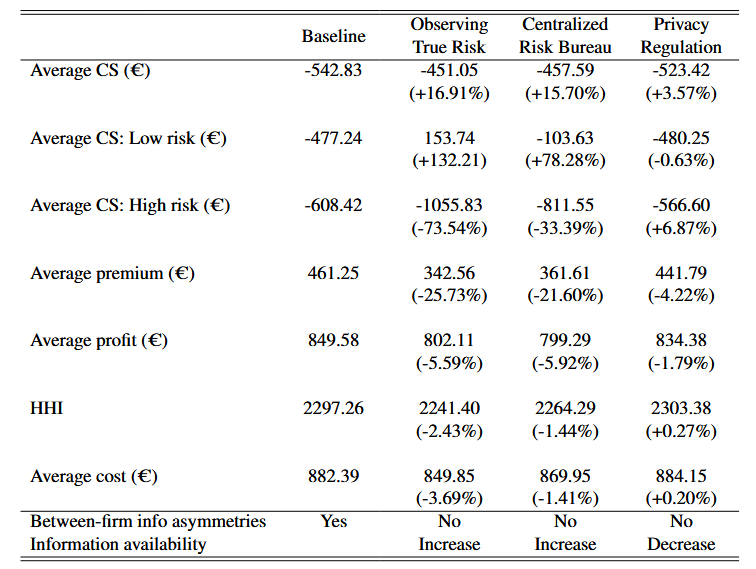
\includegraphics[scale=0.57]{Figures/Tab5.png}
\end{tabular}
\end{figure}
\end{frame}

% 28 - Change in firm profits
\begin{frame}{Change in firm profits}
\begin{columns}[t]
\begin{column}{0.44\textwidth}
\begin{itemize}
  \item Equalizing information weakens market power of precise firms.  %Precise firms lose their market power and have to compete in prices. 
  \item Common risk evaluation $\Rightarrow$ more effective undercutting $\Rightarrow$ stronger price competition.
  \item Perfect correlation in signals (uniform risk evaluation) leads to higher price competition.
\end{itemize}
\end{column}
\begin{column}{0.51\textwidth}
\vspace{-0.3cm}
\begin{figure}[H]
\centering
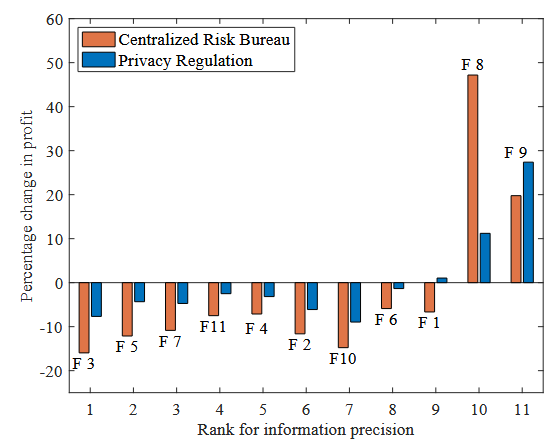
\includegraphics[width=\textwidth]{Figures/Fig5.png}
\end{figure}
\end{column}
\end{columns}
\end{frame}

% 29 - Sorting patterns
\begin{frame}{Who goes where? Sorting patterns}
\begin{columns}[t]
\begin{column}{0.44\textwidth}
\begin{itemize}
  \item With equal access to risk, firms more efficient at processing claims re-target higher-risk consumers.
  \item Sorting shifts from info advantages (baseline) to cost specialization (bureau). \\
  $\rightarrow$ increases efficiency, avg cost $\downarrow$ by $\sim$3.7\% 
  \item Sorting is lowest under privacy regulation. 
\end{itemize}
\end{column}
\begin{column}{0.51\textwidth}
\vspace{-0.3cm}
\begin{figure}[H]
\centering
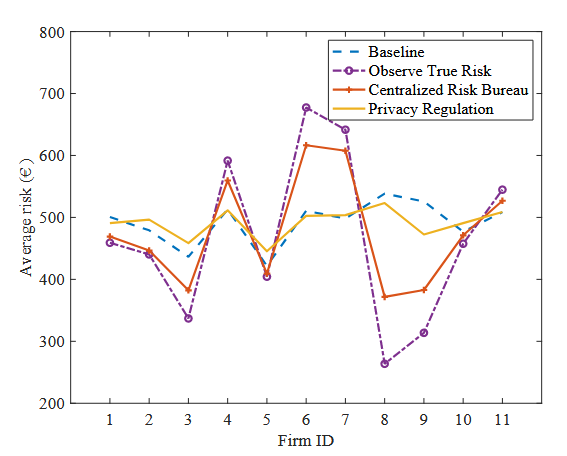
\includegraphics[width=\textwidth]{Figures/Fig6.png}
\end{figure}
\end{column}
\end{columns}
\end{frame}

% 30 - Conclusion and Comments
\begin{frame}{Conclusion}
\begin{itemize}
  \item This paper develops empirical framework for studying competition under information assymetries 
  \item This paper studies the impacts of a credit bureau, it finds: 
  \begin{itemize}
    \item Centralized information can  lower prices, raise consumer surplus and reorient sorting toward cost efficiency.
  \item Distributional trade-offs: low-risk consumers gain more under information sharing; high-risk under privacy.
  \item Industry composition effects: advanced-screening firms lose profits; potential dynamic innovation effects.
\end{itemize}
\end{itemize}
\end{frame}

% 31 - Comments
\begin{frame}{Comments }
\begin{itemize}
  \item What is the impact of a credit bureau on a dynamic world with learning-switching costs? 
  \begin{itemize}
    \item Cost of risk missclassification is low -> can update prices. 
    \item $c_j$ should be risk specific to capture inertia? 
  \end{itemize}
  \item What is a credit bureau doing in the model 
  \begin{itemize}
    \item Pooling Data: if there are economies of scale, what is the market failure? 
    \item Sharing algorithms: impact of investment in algorithms. 
  \end{itemize}
\end{itemize}
\end{frame}



%%%%%%%%%%%%%%%%%%%%%%%%%%%%%%%%%%%%%%%%%%%%%%%%%%%
\section{Appendix}
\begin{frame}{Identification of Risk Types}\label{appendix:slide1}
\begin{itemize}
  \item Risk type $\theta_i = \underbrace{\mu}_{\text{claim size}} \underbrace{\lambda_i}_{\text{accident rate}}$, 
  \item Claim size $\mu$ estimated via regression 
  \item Accident rate $\lambda_i$ (latent variable) identified from panel of accident counts (repeated noisy measurements)
   
  \item Observe accident counts $y_{it}$ over $T$ periods: $y_{it} \sim \text{Poisson}(\lambda_i)$
  \item Joint distribution of counts identifies $f(\lambda_i | p_i, D_i=j)$:
    \[
    f(y_{i1}, y_{i2}, \ldots, y_{iT} | p_i, D_i=j) = \int \prod_{t=1}^{T} \frac{\lambda_i^{y_{it}} e^{-\lambda_i}}{y_{it}!} f(\lambda_i | p_i, D_i=j) d\lambda_i
    \]
    \item Output  $\hat{g}(p | \theta, D=j)$ for demand estimation 
    \hyperlink{estimation:overview}{\beamergotobutton{Go back}}
\end{itemize}
\end{frame}

\begin{frame}{Conditional choice probabilities}\label{appendix:slide2}
\begin{itemize}
  \item Demand is produced by the model: 
  
  \[
  \Pr(D=j|p_j=p, \theta) = \int_{\mathbf{p}_{-j}} \frac{\exp(-\gamma p + \xi_j)}{\exp(-\gamma p + \xi_j) + \sum_{j' \ne j} \exp(-\gamma p_{j'} + \xi_{j'})} \left( \prod_{j' \ne j} g_{j'}(p'_{j'}|\theta) \right) d\textbf{p}_{-j}.
  \]
    \hyperlink{estimation:demand}{\beamergotobutton{Go back}}
\end{itemize}
\end{frame}

\begin{frame}{Identification of Pricing Coefficients ($\alpha_j, \beta_j$)}\label{appendix:slide3}
\begin{itemize}
  \item Pricing strategy: $p_j(\hat{\theta}_j) = \alpha_j + \beta_j E(\theta|\hat{\theta}_j, D=j)$
  \item \textbf{Key Insight:} Linear structure allows identification from first and second moments
  \item \textbf{Objects already recovered:} within-firm offered-price density $g_j(p\mid\theta)$ 
\end{itemize}

\textbf{Within-firm moments:} 
$$\text{Mean premium:} \quad  E(p|D=j) = \alpha_j + \beta_j E(E(\theta|\hat{\theta}_j, D=j)|D=j) = \alpha_j + \beta_j E(\theta|D=j) $$
\vspace{-.3cm}
$$\text{Premium and Risk covariance:} \quad  \text{cov}(p, \theta|D=j) = \beta_j \text{var}(E(\theta|\hat{\theta}_j, D=j)|D=j) = \frac{\text{var}(p|D=j)}{\beta_j} $$


\vspace{0.2cm}

\textbf{Solution:} Solve system of two linear equations
{\small
\[
\beta_j \;=\; \frac{\operatorname{var}(p\mid D=j)}{\operatorname{cov}(p,\theta\mid D=j)},
\qquad
\alpha_j \;=\; \mathbb{E}(p\mid D=j)\;-\;\beta_j\,\mathbb{E}(\theta\mid D=j),
\]
}

\textbf{Advantage:} estimated separately from other parameters $\rightarrow$ reduces computational burden\hyperlink{estimation:overview}{\beamergotobutton{Go back}}

\end{frame}


\begin{frame}{Identification of Signal Variance ($\sigma_j$)}\label{appendix:slide3.1}

\begin{itemize}
  \item \textbf{Key Insight:} monotonicity of prices on the signal (similar to GPV(2000))
\end{itemize}

\begin{enumerate}
  \item Using monotonicity and then inverting: {\small
$$ G_j(p_j(\hat{\theta}_j)|\theta) = \Phi\left(\frac{\hat{\theta}_j - \theta}{\sigma_j}\right) \implies p_j^o(\hat{\theta}_j; \theta, \sigma_j) = G_j^{-1}\left(\Phi\left(\frac{\hat{\theta}_j - \theta}{\sigma_j}\right)\right)$$
}

where $G_j(p|\theta)$ = CDF of offered prices (recovered from demand estimation)

\item For a given $\sigma_j$, evaluate risk rating at equilibrium prices: 
 {\small
$$ E(\theta|\hat{\theta}_j, D=j; \sigma_j) = \frac{\int_\theta \theta \Pr(D=j|p_j^o(\hat{\theta}_j; \theta, \sigma_j), \theta) \phi(\hat{\theta}_j; \theta, \sigma_j) f_0(\theta) d\theta}{\int_\theta \Pr(D=j|p_j^o(\hat{\theta}_j; \theta, \sigma_j), \theta) \phi(\hat{\theta}_j; \theta, \sigma_j) f_0(\theta) d\theta} $$
}

\item Using $p_j(\hat{\theta}_j; \sigma_j) = \hat{\alpha}_j + \hat{\beta}_j E(\theta|\hat{\theta}_j, D=j; \sigma_j)$ obtain the model-implied joint distribution of $(p, \theta)$ within firm $j$ 

\item Match model implied dist. of $(p, \theta)$ to the empirical dist. recovered from the data. 
\end{enumerate}
\end{frame}


\begin{frame}{Supply parameters: $c_j, k_j$}\label{appendix:slide4}
  
\textbf{Net profit from servicing consumer:} $p_j(\hat{\theta}_j) + c_j - k_j\theta$

\begin{itemize}
    \item $c_j$ = net benefit from contracting (inertia, dynamic pricing, cross-selling)
    \item $k_j\theta$ = claim processing cost (efficiency parameter $k_j$ times expected claims)
\end{itemize}

\vspace{0.3cm}

\textbf{First-Order Conditions:} Firm $j$ optimally chooses $(\alpha_j, \beta_j)$

{\small
\[
\frac{\partial\pi_j}{\partial \alpha_j}
=\int_\theta\!\!\int_{\hat{\theta}} \Pr(D=j\mid \hat\theta,\theta)\,f(\hat\theta\mid\theta)f_0(\theta)\,d\hat\theta\,d\theta
+\int_\theta\!\!\int_{\hat{\theta}} (\alpha_j+\beta_j\theta+c_j-k_j\theta)\,
\frac{\partial \Pr(D=j\mid \hat\theta,\theta)}{\partial \alpha_j}\,f(\hat\theta\mid\theta)f_0(\theta)\,d\hat\theta\,d\theta,
\]
\[
\frac{\partial\pi_j}{\partial \beta_j}
=\int_\theta\!\!\int_{\hat{\theta}} \theta\,\Pr(D=j\mid \hat\theta,\theta)\,f(\hat\theta\mid\theta)f_0(\theta)\,d\hat\theta\,d\theta
+\int_\theta\!\!\int_{\hat{\theta}} (\alpha_j+\beta_j\theta+c_j-k_j\theta)\,
\frac{\partial \Pr(D=j\mid \hat\theta,\theta)}{\partial \beta_j}\,f(\hat\theta\mid\theta)f_0(\theta)\,d\hat\theta\,d\theta.
\]
}

\vspace{0.2cm}

\textbf{Solution:} Given previously recovered $\{g_j,\,E(\theta\mid\hat\theta_j,D=j),\,\alpha_j,\,\beta_j,\,\sigma_j\}$ and $\Pr(D=j\mid\cdot)$, it is a system of 2 linear equations in $(c_j, k_j)$ where all other terms are known \hyperlink{estimation:overview}{\beamergotobutton{Go back}}
\end{frame}
 
\end{document}
